%  -----------------------------------------------------------------------------
%  Author         : Bimalka Piyaruwan Thalagala
%  GitHub         : https://github.com/bimalka98
%  Date Created   : 01.09.2020
%  Last Modified  : 15.02.2020
%  -----------------------------------------------------------------------------

\documentclass[a4paper,11pt]{article}%,twocolumn
\input{settings/packages}
%% page settings
\usepackage[top=10mm, bottom=15mm,left=10mm,right=10mm]{geometry}  
 % needed for page border settings
\parindent=0mm % for space of first line of new text block

\sloppy % for writing with hyphenless justification (tries to)
\hyphenation{} % use hyphenation of tolerance parametershttp://www.jr-x.de/publikationen/latex/tipps/zeilenumbruch.html
\hyphenpenalty=10000
\exhyphenpenalty=10000
\usepackage{fancyhdr} % needed for head and foot options
\input{settings/jupyter}


\begin{document}


\begin{titlepage}
\center % Center everything on the page

%-------------------------------------------------------------------------------------
%	HEADING SECTIONS
%------------------------------------------------------------------------------------
\textbf{\large Department of Electronic and Telecommunication Engineering}\\[0.5cm]
\textbf{\Large University of Moratuwa, Sri Lanka}\\[1cm]
\textbf{\large EN2550 - Fundamentals of Image Processing and Machine Vision}\\[2cm]
\includegraphics[width=0.3\textwidth]{figures/uomlogo}\\[2cm]

	
%-------------------------------------------------------------------------------------
%	TITLE SECTION
%------------------------------------------------------------------------------------
\textbf{\Huge Assignment 01}



%----------------------------------------------------------------------------------------
%	MEMBERS SECTION
%----------------------------------------------------------------------------------------

\vfill

\textbf{\large Submitted by}\\[0.5cm]

{\large Thalagala B.P.}	\hspace{5mm} {\large 180631J }\\[1cm]

%----------------------------------------------------------------------------------------
%	DATE SECTION
%----------------------------------------------------------------------------------------

\textbf{\large Submitted on}\\[0.5cm]
\textbf{\Large \today} % Date, change the \today to a set date if you want to be precise

%----------------------------------------------------------------------------------------

 % Fill the rest of the page with whitespace

\end{titlepage}
\tableofcontents

\begin{center}
	\textbf{\textit{* PDF is clickable}}
\end{center}

\pagebreak
\section{Part 1: Basic Operations}
\subsection{Histogram computation and Histogram equalization}
\begin{figure}[!h]
	\centering
	\subfigure[Original Image]
	{ \includegraphics[scale=0.2]{figures/img0}

	}
	\subfigure[Hist: of the Original Image]
	{ 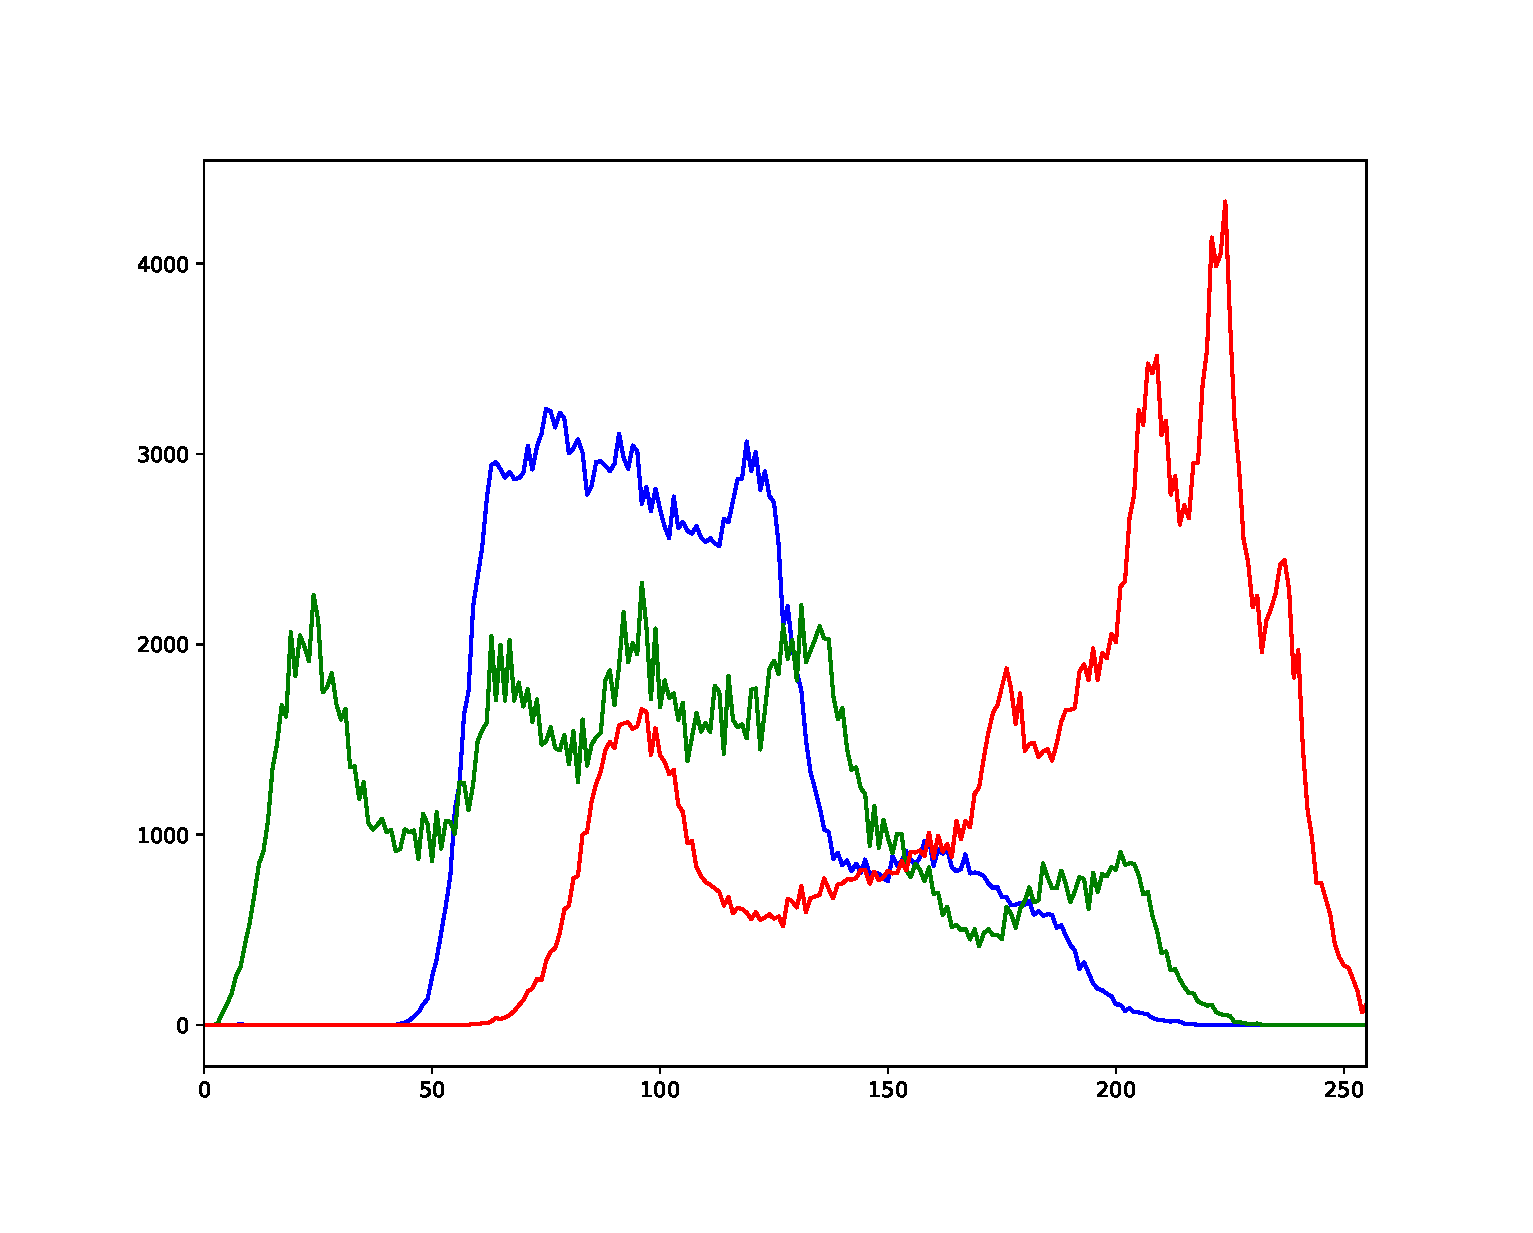
\includegraphics[scale=0.2]{figures/hiscomp}

	}
	\subfigure[Hist: Equalized Image]
	{ \includegraphics[scale=0.2]{figures/equalized_img}

	}
	\subfigure[Equalized Histogram]
	{ 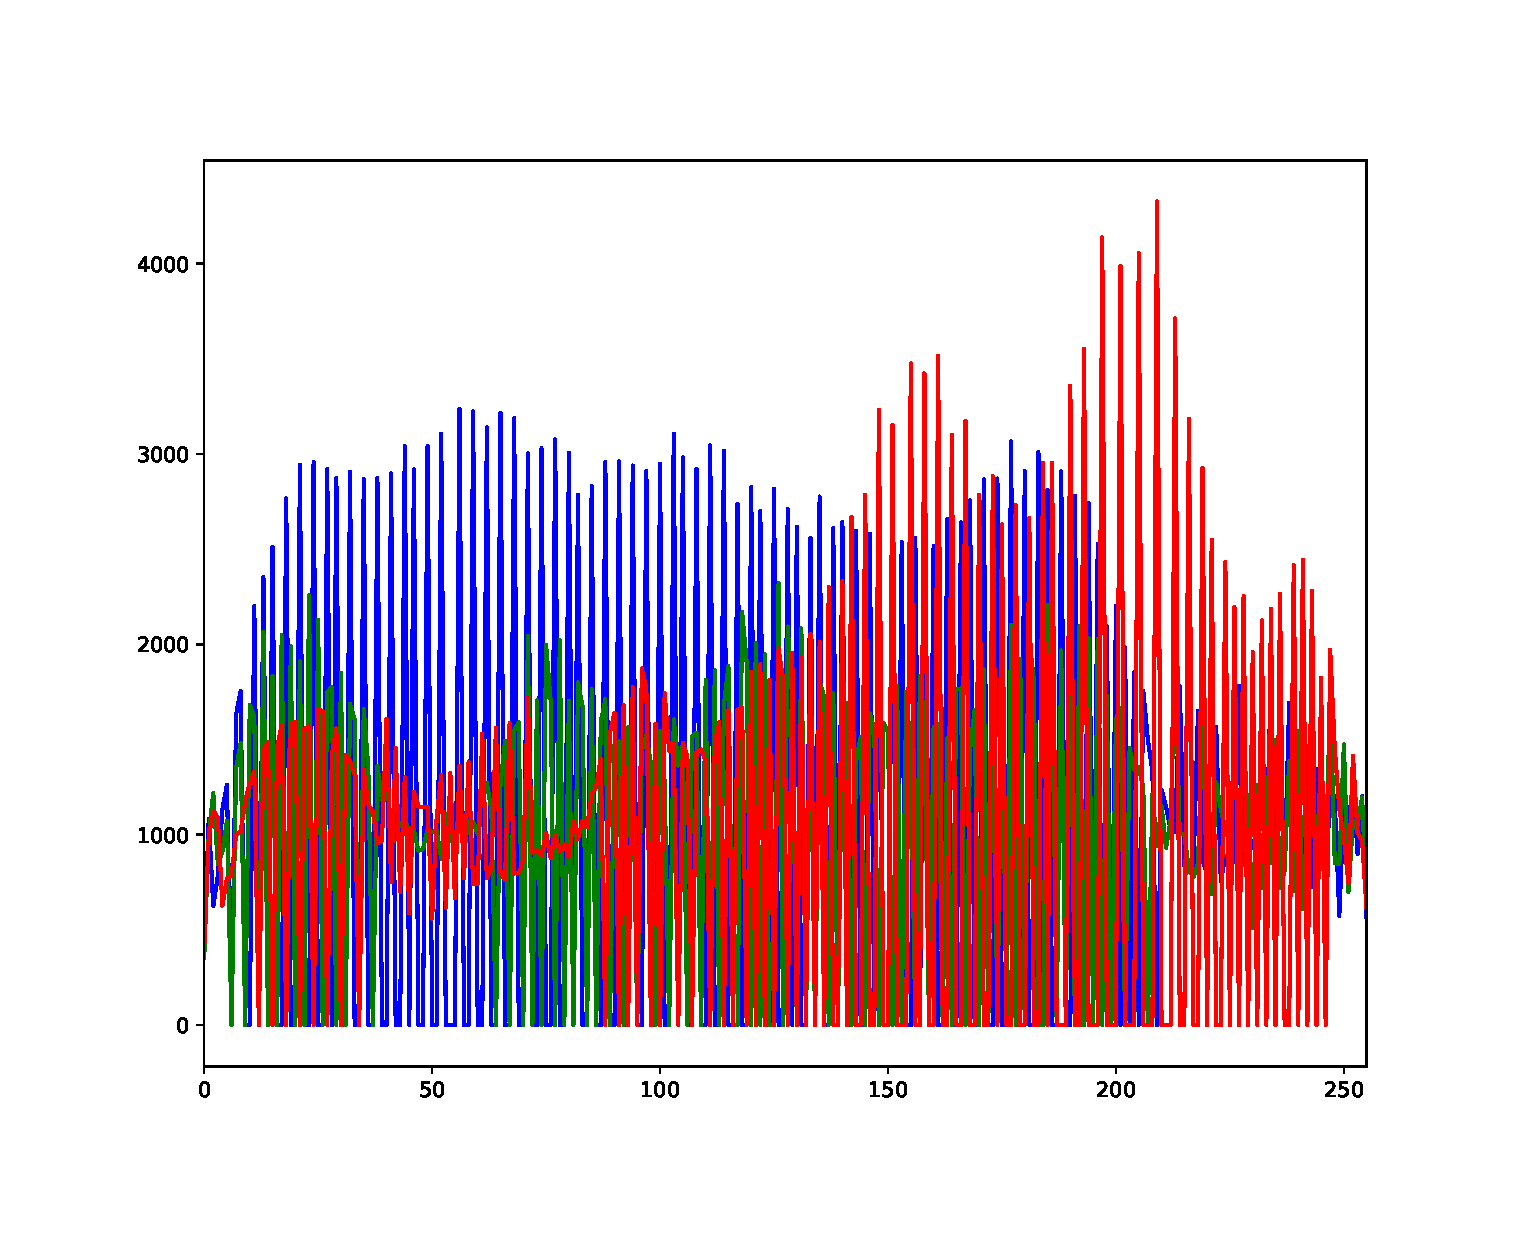
\includegraphics[scale=0.2]{figures/hisequ}

	}
\caption{caption goes here}
\end{figure}




\subsection{Intensity transformations}

\begin{figure}[!h]
	\centering
	\subfigure[Original Image]
	{ \includegraphics[scale=0.2]{figures/boriginal}

	}
	\subfigure[Transformation]
	{ 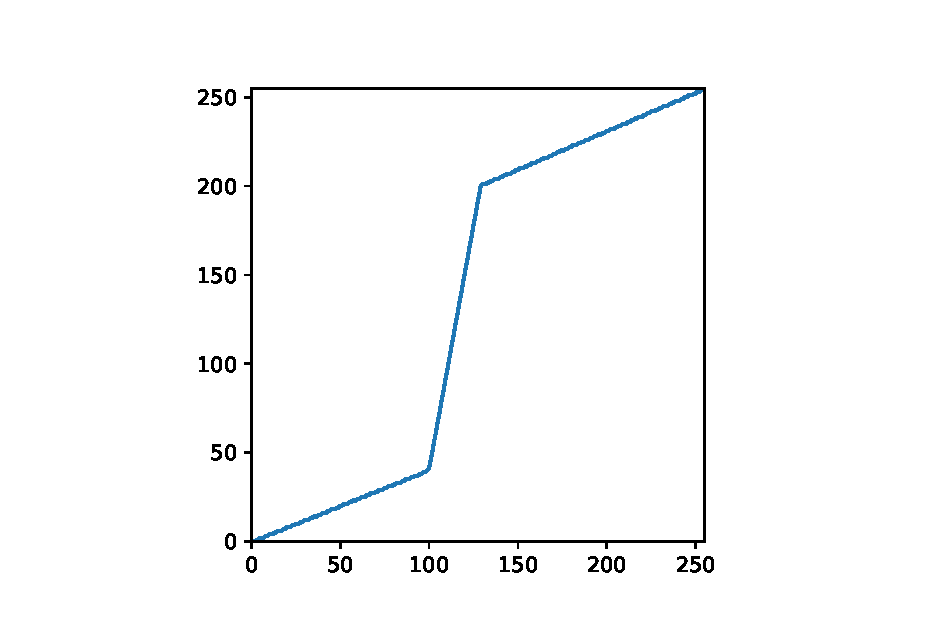
\includegraphics[scale=0.4]{figures/transformation}

	}
	\subfigure[Transformed Image]
	{ \includegraphics[scale=0.2]{figures/btransformed}

	}
\caption{caption goes here}
\end{figure}






\subsection{Gamma correction}

\begin{figure}[!h]
	\centering
	\subfigure[Gamma Corrected Image $\gamma = 1.3$]
	{ \includegraphics[scale=0.2]{figures/dgamma3}

	}
	\subfigure[Original Image  $\gamma = 1$]
	{ \includegraphics[scale=0.2]{figures/doriginal}

	}
	\subfigure[Gamma Corrected Image $\gamma = 0.7$]
	{ \includegraphics[scale=0.2]{figures/dgamma7}

	}
		\subfigure[Gamma Corrected Image $\gamma = 0.4$]
	{ \includegraphics[scale=0.2]{figures/dgamma4}

	}
\caption{caption goes here}
\end{figure}





\subsection{Gaussian smoothing $\sigma = 1.5$}

\begin{figure}[!h]
	\centering
	\subfigure[Original Image]
	{ \includegraphics[scale=0.45]{figures/eoriginal}

	}
	\subfigure[Kernel Size = 7]
	{ \includegraphics[scale=0.45]{figures/SmoothkernelS7}

	}
	\subfigure[Kernel Size = 13]
	{ \includegraphics[scale=0.45]{figures/SmoothkernelS13}

	}
	\subfigure[Kernel Size = 21]
	{ \includegraphics[scale=0.45]{figures/SmoothkernelS21}

	}
\caption{caption goes here}
\end{figure}




\subsection{Unsharp masking}

\begin{figure}[!h]
	\centering
	\subfigure[Original Image]
	{ \includegraphics[scale=0.25]{figures/foriginal}

	}
	\subfigure[Gaussian Blurred]
	{ \includegraphics[scale=0.25]{figures/blurred}

	}
	\subfigure[Mask + 125]
	{ \includegraphics[scale=0.25]{figures/mask}

	}
	\subfigure[Sharpened Image]
	{ \includegraphics[scale=0.25]{figures/sharpened}

	}
\caption{caption goes here}
\end{figure}



\subsection{Median filtering }

\begin{figure}[!h]
	\centering
	\subfigure[Original Image]
	{ \includegraphics[scale=0.23]{figures/goriginal}

	}
	\subfigure[Adding Salt \& Pepper Noise]
	{ \includegraphics[scale=0.23]{figures/saltpepper}

	}
	\subfigure[Kernel Size = 3]
	{ \includegraphics[scale=0.23]{figures/medianfilterimage3}

	}
	\subfigure[Kernel Size = 5]
	{ \includegraphics[scale=0.23]{figures/medianfilterimage5}

	}
\caption{caption goes here}
\end{figure}


\subsection{Bilateral filtering}

Bilateral filter extends the idea of Gaussian smoothing by adding \textbf{\textit{edge preserving capability}} which is not possible in the Gaussian filtering because there, only the Spatial distance to the pixels' from the central pixel were considered when applying the weights(Same Gaussian kernel everywhere) and therefore \textbf{\textit{Gaussian filter averages across the edges}}. Assuming that pixels' intensity value do not change rapidly over the window. As a consequence the same weight is applied to a pixel on an edge(say high intensity) and a pixel near an edge(say low intensity) when calculating the central pixel's value.\\

In the bilateral filter \textbf{\textit{intensities of the neighborhood pixels are also considered}} when applying the weight in addition to the spatial distance. This makes it possible to \textbf{\textit{eliminate the averaging across edges}}. As following figures shows when $\sigma_r$ approaches $\infty$, bilateral filter gives the result of the Gaussian filter. Here $\sigma_s$ is spatial deviation(spatial extent of the kernel) while $\sigma_r$ is the color space deviation(minimum amplitude of an edge).



\begin{figure}[!h]
	\centering
	\subfigure[Original Image]
	{ \includegraphics[scale=0.37]{figures/horiginal}

	}
	\subfigure[Gaussian Kernel Size = 9, $\sigma_s=6$]
	{ \includegraphics[scale=0.37]{figures/gaussianB}

	}
	\subfigure[Bilateral Kernel Size = 9, $\sigma_s = 6$, $\sigma_r = 100$ ]
	{ \includegraphics[scale=0.37]{figures/bl5}
	}
	\subfigure[Bilateral Kernel Size = 9, $\sigma_s = 6$, $\sigma_r = 10$]
{ \includegraphics[scale=0.37]{figures/bl9}
}
\caption{Bilateral filtering}
\end{figure}



\section{Part 2: Count the rice grains in the rice image}

The objective of counting the rice grains can be achieved through binary segmentation since we have only two different object types namely rice grains and the background. Since the image has different lighting conditions, \textbf{\textit{adaptive thresholding}} must be used. To get rid of the unwanted white noise in the background and to detach connected grains \textbf{\textit{erosion morphological transformation}} is used(Rectangular kernel is used over elliptic and cross shape kernels since it was found to be the best at achieving the goals).

\begin{figure}[!h]
	\centering
	\subfigure[Gray Scale Image]
	{ \includegraphics[scale=0.38]{figures/part2/2original}
	}
	\subfigure[Adaptive Thresholding]
	{ \includegraphics[scale=0.38]{figures/part2/img_adapt_thresh}
	}
	\subfigure[Erosion]
	{ \includegraphics[scale=0.38]{figures/part2/eroded_img}
		}
	\subfigure[Connected Components]
	{ \includegraphics[scale=0.38]{figures/part2/labeledImg}
	}
	\subfigure[Color Mapped Image]
	{ \includegraphics[scale=0.38]{figures/part2/imgColorMap}
	}
	\caption{Counting the rice grains}
\end{figure}



\section{Part 3: Zoom Images}


%---------------------------------------------------------------------------
\end{document}
